\subsubsection*{The Codegenerator Visitor}
When the code generator is called from the \texttt{main()} class, uses the \acrshort{ast} to accept a \texttt{CodeGeneratorVisitor} as seen on \myref{fig:CodeGeneratorVisitor}.

\begin{figure}[!ht]
\centering
 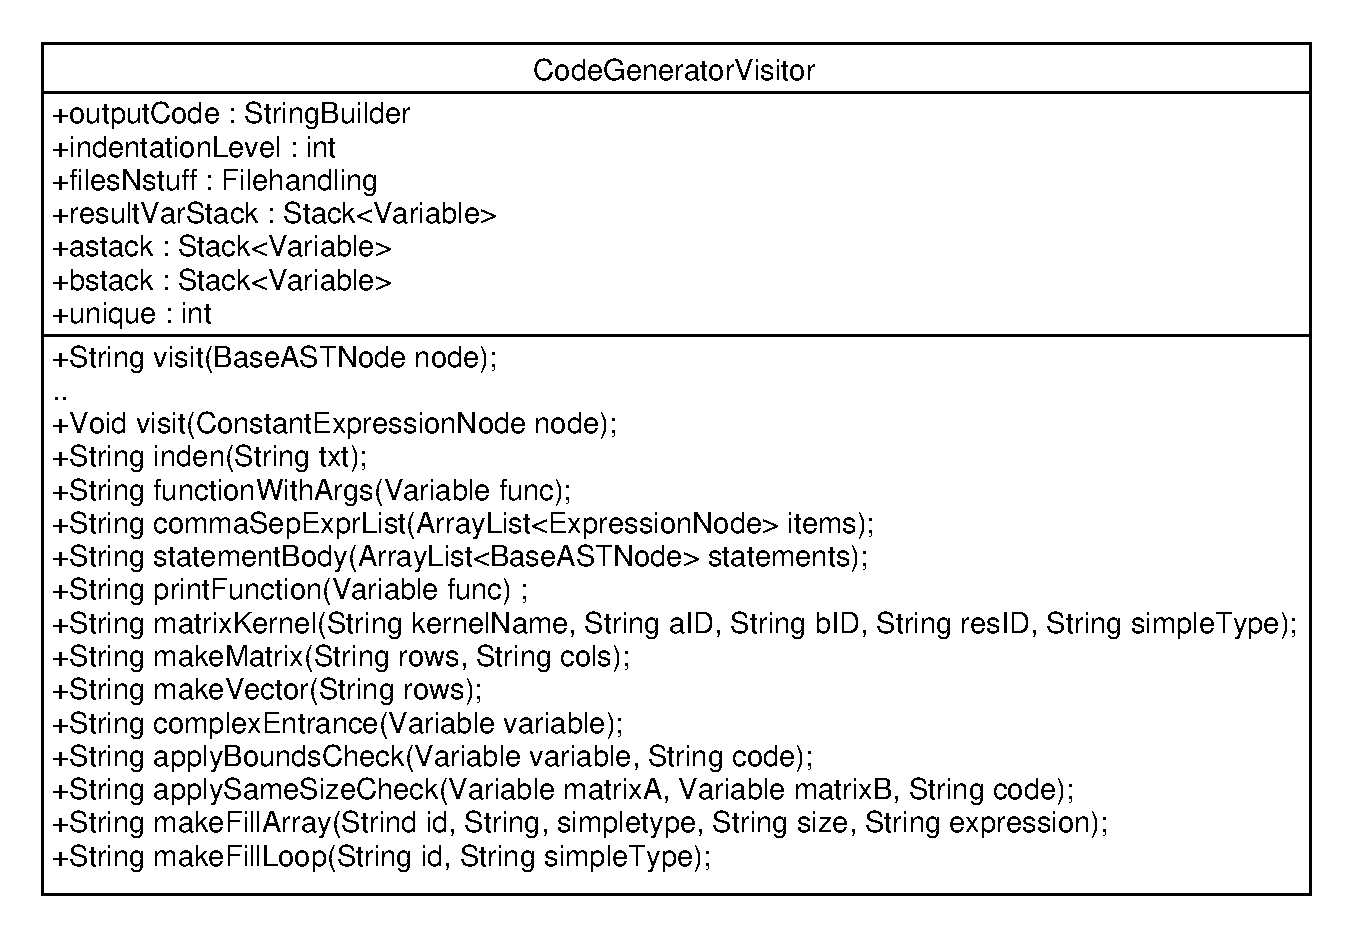
\includegraphics[width=1\textwidth]{figures/ClassDiagrams/CodeGeneratorCall.pdf} % trim=4.85cm 15cm 0.85cm 1cm
\caption{A diagram showing the call from the code generator to the visitor which makes the string from the decorated \acrshort{ast}.}\label{fig:CodeGeneratorVisitor}
\vspace{-15pt}
\end{figure}

The visitor builds a string by traversing the nodes of the tree.
Simpler visit methods like a visit method for a \texttt{ConstantExpressionNode} returns a string.
The string is then used in other visit methods e.g. \texttt{AssignmentNode} which then creates a string which is a statement that can be executed in C.
This string from \texttt{AssignmentNode} is then appended to the string, which will contain the outputcode for the \gls{gamble} program when all the nodes from the decorated \acrshort{ast} has been visited.

This means that the information bubbles upwards from the leafs to the statementnodes.
The information ends up in the correct statementnodes  because the visitor pattern makes it possible to specify the route of traversal.
The \texttt{CodeGeneratorVisitor} also contains other methods for making certain C constructions from the \acrshort{ast} which can also be seen on \myref{fig:CodeGeneratorVisitor}.
Some of these functions also make runtime checks of matrices, as matrices needs to be of compatible sizes for some of the operations which can be performed on a matrix.
If multiplying 2 matrices the left matrix of the multiplication has to be a nxm while the right one has to be a mxp matrix.
So the right matrix has to have the same number of columns as the right matrix has rows.
If performing a matrix index multiplication, where every index is multiplied with the corresponding index of the the other matrix, the matrices have to have the same number of rows and columns.

These checks will be inserted as a surrounding if statement around the matrix calculations, so they have to pass these checks before the calculation will be done.
The reason this is done at run-time instead of compile-time is because the sizes of matrices can be dynamic, which results in making it impossible to check for this at compile-time.

When the string is complete it is printed into a file called code.c, along with all the other files needed for running the code, e.g. the kernels used for performing computations on the \acrshort{gpu}.

